d\chapter{Introduction}
\label{sec:intro}
\chaptermark{Optional running chapter heading}

Introduction.

This is a subsection.

% \begin{figure}[t]
% \centering
% 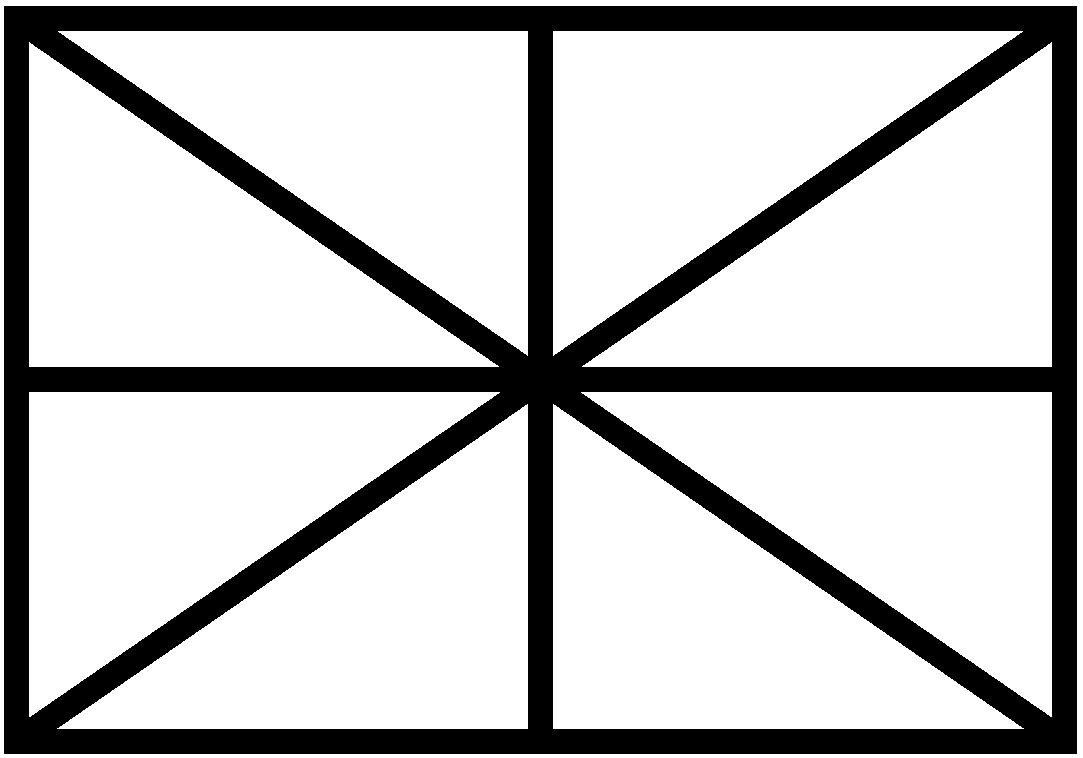
\includegraphics[width=\textwidth]{figure}
% \makeatletter
% \let\@currsize\normalsize
% \caption{Caption.}
% \label{fig:figure}
% \end{figure}
% 
% \begin{figure}[t]
% \centering
% \begin{tabular}{c c}
% \includegraphics[height=2.5in]{figureA} &
% \includegraphics[width=3in]{figureB}\\
% (A) & (B)
% \end{tabular}
% \makeatletter
% \let\@currsize\normalsize
% \caption{Two figures.}
% \label{fig:twofigures}
% \end{figure}

% currsize is not set in the long table environment, so we need to set it before we set it up.
\makeatletter
\let\@currsize\normalsize
\makeatother


\noindent Again, we don't indent here.